\chapter{Generative Adversarial Networks} \label{cha:gans}
\glsunset{GAN}

\acp{GAN} fall into a particular subfield of machine learning called \textit{generative modeling}, the goal of this area of study is to be able to generate original data based on a training dataset. As mentioned in \autoref{sub:unsupervised_learning}, the data found in real life scenarios for any given situation is just a very tiny fraction of all the possible values in the input space, recall the \gls{MNIST} example given, just a minuscule subset of all possible images can be sensibly interpreted as digits. It can be said that real world data has some structure, and generative models aim to replicate this structure in order to sample from it.


\section{Generative Models and Data Distributions}
\textcite{nipsGAN2017} explains that any dataset is made of samples taken from some probability distribution $p_{data}$ that defines the structure of the data, and all the different techniques in generative modeling are trying to produce a $p_{model}$ to replicate as close as possible the underlying distribution of the data.

If $p_{data}$ was known for a given problem, then it could be used by itself to generate original data, but calculating this distribution is basically impossible for all but the simplest datasets, so the most a model can do is try to replicate it. To better understand the complexities in probability distributions it can be helpful to look at some characteristics in the, relatively simple, \gls{MNIST} dataset.

Recall that the \gls{MNIST} dataset consists of $70,000$ grayscale images of size $28\times28$, and these images are color inverted. When introducing the dataset in \autoref{sec:mnist} the images were inverted again to show the original colors, but here the properties will be analyzed without making any preprocessing on the data. First it is helpful to look at what is the mean and variance for each pixel in the \gls{MNIST} dataset, these values are shown in \autoref{fig:mnist_mean_var}.
\begin{figure}[h]
    \centering
    \caption{\gls{MNIST} mean and variance}
    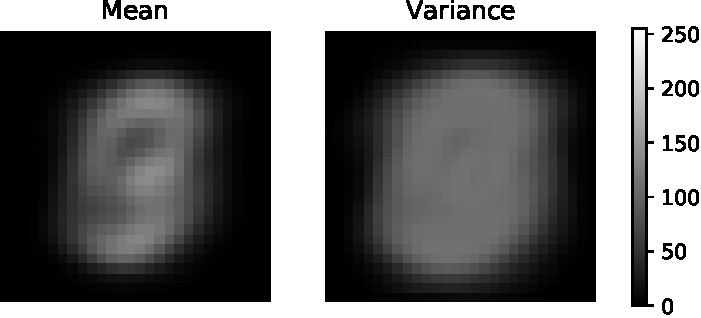
\includegraphics[width=0.65\textwidth]{chapters/GANs/figures/mnist_mean_var.pdf}
    \fonte{From the author (2021)}
    \label{fig:mnist_mean_var}
\end{figure}

The information in \autoref{fig:mnist_mean_var} already gives some insight into how the data is structured, the edges of the image practically see no change since all the digits are centered, and it is possible to see dips in brightness in the middle-top and middle-bottom of the digits; these represent the spaces that all the digits are drawn around (i.e. the two holes in the number $8$).

Another way to see the distribution is to directly plot the probability of seeing the different values for a pixel, this is done by counting how many times each value has appeared in a selected pixel for all images in the dataset, the probability is then the number of value occurrences divided by the total number of images. Doing this for one of the center pixels, in row 15 and column 15, the end result is the probability distribution seen in \autoref{fig:mnist_pixel_dist}.
\begin{figure}[hbt]
    \centering
    \caption{Probability distribution of values in pixel (15,15) of \gls{MNIST}}
    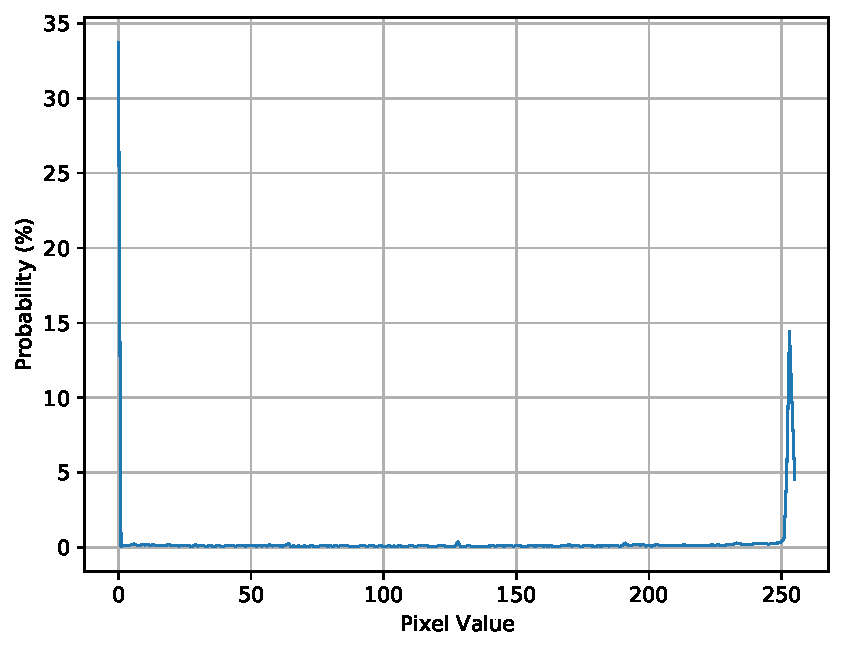
\includegraphics[width=0.6\textwidth]{chapters/GANs/figures/mnist_dist_pixel_14x14.pdf}
    \fonte{From the author (2021)}
    \label{fig:mnist_pixel_dist}
\end{figure}

The probability distribution in \autoref{fig:mnist_pixel_dist} gives even more information about the dataset, it can be seen that the values are either completely black, or a very bright white. Any grayish values are very unlikely since with handwriting digits the strokes are very sharp and well defined. It is possible to extend \autoref{fig:mnist_pixel_dist} by calculating the distribution for a whole column of pixels, the result is a 3D surface, where the new axis represents the corresponding pixel in the column. \autoref{fig:mnist_column_dist} shows this surface for columns 2 and 15 of the \gls{MNIST} dataset, note that the digit besides the shape is there only to illustrate the position of the column, the distribution is for the entire dataset.
\begin{figure}[hbt]
    \centering
    \caption{Probability distribution of values in columns of \gls{MNIST}}
    \begin{subfigure}{0.7\textwidth}
        \centering
        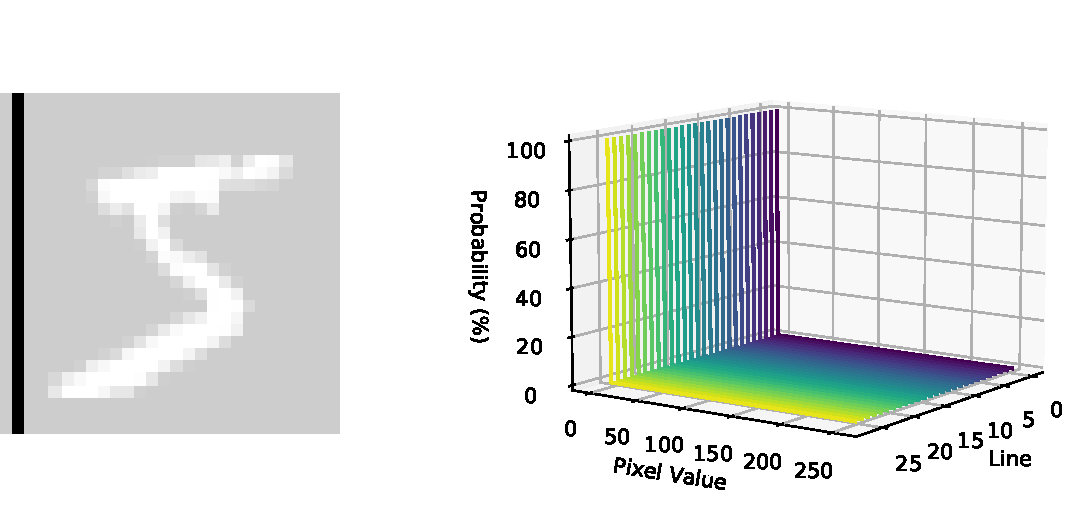
\includegraphics[width=\textwidth]{chapters/GANs/figures/mnist_highlight_dist_column_1.pdf}
        \caption{Column 2}
    \end{subfigure}
    
    \begin{subfigure}{0.7\textwidth}
        \centering
        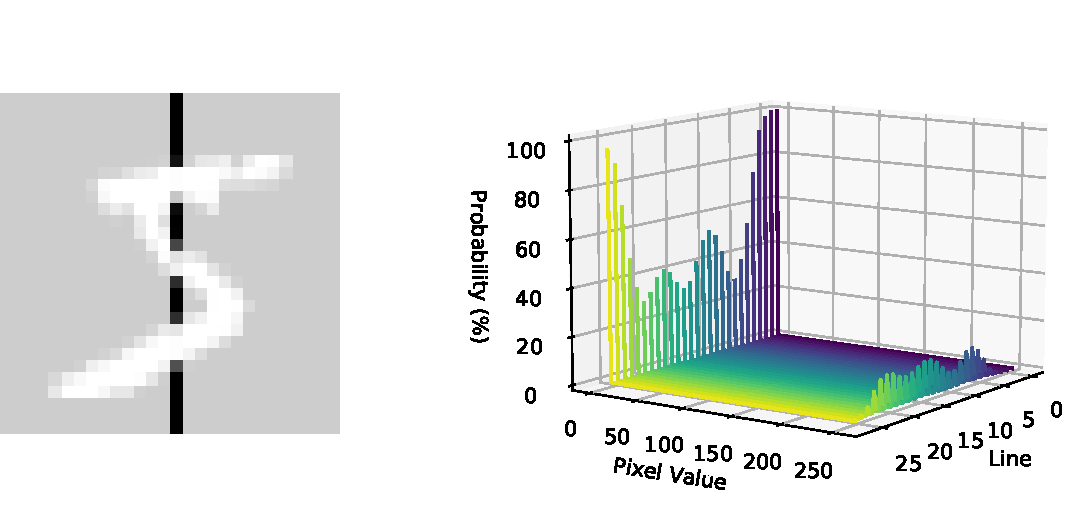
\includegraphics[width=\textwidth]{chapters/GANs/figures/mnist_highlight_dist_column_14.pdf}
        \caption{Column 15}
    \end{subfigure}
    
    \fonte{From the author (2021)}
    \label{fig:mnist_column_dist}
\end{figure}

The probabilities shown in \autoref{fig:mnist_column_dist} reinforce what was seen for the mean and variance of the images in \autoref{fig:mnist_mean_var}, for the edges the probability is basically 100\% that a pixel will be completely black, while for the center column it is possible to see the probabilities being split into very dark or very light pixel values, it even has two slight peaks for the black pixels representing the spaces between the digits (i.e. the holes in the number $8$) as also seen for the mean and variance case.

One may think that this would be enough to represent and generate new data, since the probability distribution for each pixel is already calculated, wouldn't all the image be described? And by sampling the distribution for each pixel, wouldn't it be possible to generate new images of digits? It is certainly possible to try, \autoref{fig:mnist_simple_sample} show three examples of images generated by sampling from the pixel distributions.
\begin{figure} [hbt]
    \centering
    \caption{Images generated by sampling from the pixel distributions of \gls{MNIST}}
    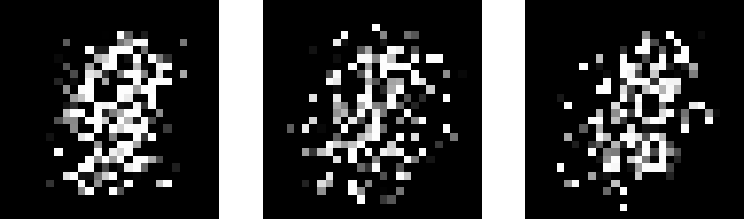
\includegraphics[width=0.8\textwidth]{chapters/GANs/figures/mnist_simple_samples.pdf}
    \fonte{From the author (2021)}
    \label{fig:mnist_simple_sample}
\end{figure}

The sampled images surely have some similarities, but they are far from being digits. Although the probability distributions calculated are very helpful in giving some insight into the dataset, they consider the pixels as completely independent from one another. In reality, neighbouring pixels influence the values of each other, for handwritten digits a pixel will practically never be white while it's neighbours are all black, instead it is much more likely that a white pixel will have some of it's neighbours also being white in order to produce a stroke in the image. By averaging out all the influences of every pixel, the resulting distributions are those seen in \autoref{fig:mnist_pixel_dist} and \autoref{fig:mnist_column_dist}; they are valid descriptions of the data, but cannot be used to fully represent the underlying structure.

The results in \autoref{fig:mnist_simple_sample} are similar to an effect seen in some neural network models, the data has many possible correct representations, but instead of picking a single one, the model averages out everything and ends up with a blurry mixture that badly represents the data. This can be seen for example in models that colorize black and white images \cite{automaticColorization2016} (e.g. averaging reds, yellows, blues and all other common car colors, results in painting most cars in the same bland sepia tones), and models that aim to increase the resolution of images \cite{ganSuperResolution2016}.

One of the advantages of \acp{GAN} is that they are more resistant to these kinds of problems, \autoref{fig:super_resolution} bellow shows an example where the original image was downscaled and different approaches were used to upscale the result back to it's original size. Note how the \gls{GAN} (called SRGAN) produces sharper results when compared with the algorithmic approach of bicubic upscaling and with another neural network that does not use a \gls{GAN} architecture (SRResNet) \textbf{--} this latter case has some understanding of the underlying structure, but it suffers to pick one good solution and instead ends up averaging all possible answers resulting in a blurry image \cite{nipsGAN2017}.
\begin{figure}[hbt]
    \centering
    \caption{Comparison of different upscaling techniques (upscaling $\times4$)}
    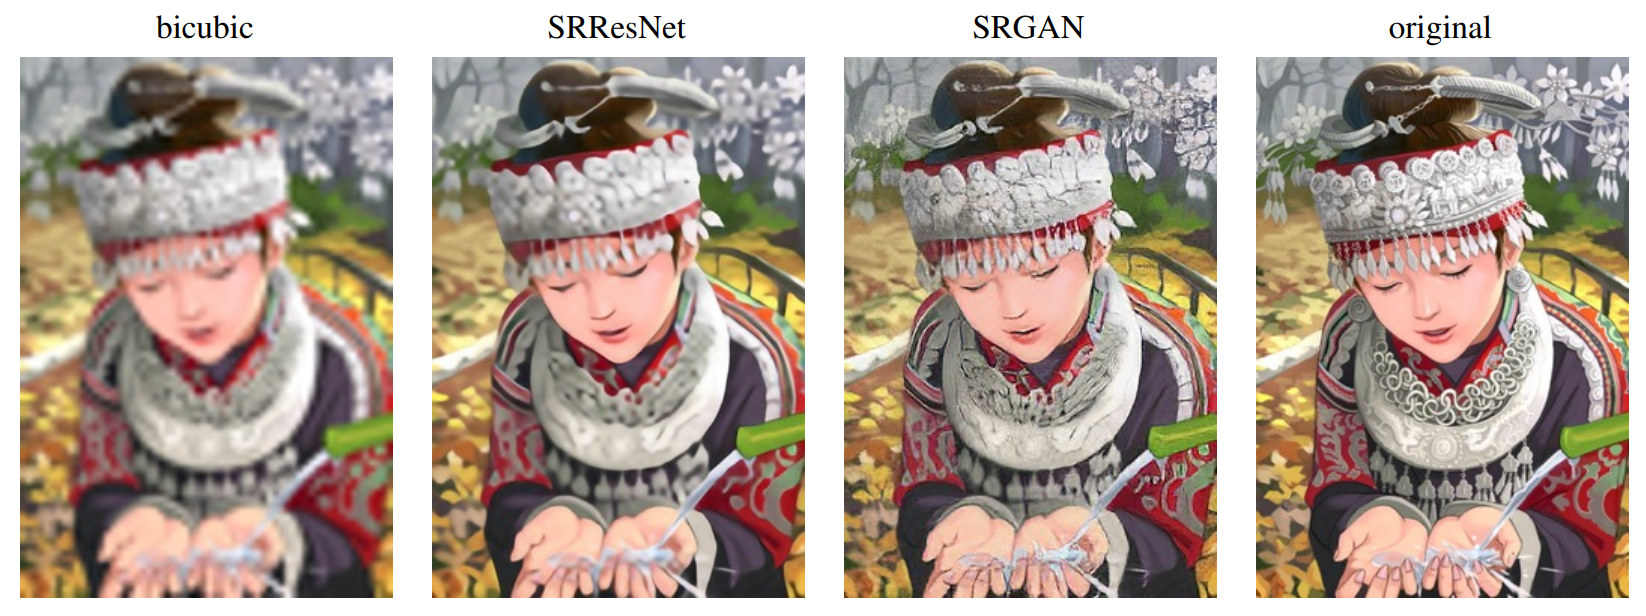
\includegraphics[width=0.9\textwidth]{chapters/GANs/figures/superResolution.png}
    \fonte{Adapted from \textcite{ganSuperResolution2016}}
    \label{fig:super_resolution}
\end{figure}

In the next section the reason why \acp{GAN} are better at this will be explored more deeply. For now these examples show how complex the probability distributions of data can be (even knowing all the probabilities for each pixel still is not enough), given this complexity it is only possible to approximate the distributions, and generative models are a way of doing that.

One may question the purpose of generative models since the idea behind them is simply to generate more of what there is already a lot of. Indeed for cases like \gls{MNIST} there is little value in generating a lot more digits, this problem has been solved since the 1990's \cite{mnist1998}, and now it only serves as a learning and benchmark tool. However the use of generative models can be extended to more diverse situations, as already seen for upscaling images in \autoref{fig:super_resolution}. \textcite{nipsGAN2017} highlights some other uses of generative models, including: different ways to incorporate these models into Reinforcement Learning, leveraging unlabelled data as seen in semi-supervised learning, image-to-image translation, and creation of art.


\section{The GAN Architecture} \label{sec:gan_architecture}
The \gls{GAN} is a type of neural network that was introduced by \textcite{gans2014} as an alternative to other generative models at the time. The main idea behind it is the competition of two different networks, a \textit{generator} and a \textit{discriminator}, hence the term \textit{Adversarial} in Generative Adversarial Network. The discriminator is trained with the simple goal of detecting if any given sample belongs or not to the original dataset. The generator on the other hand is trained to make the discriminator fail, it's goal is to create samples that the discriminator will consider real.

A common analogy given for this process is that of the police trying to identify counterfeit money \cite{nipsGAN2017}, the generator in this analogy is the criminals, and the discriminator is the police. The criminals will start making bad replicas that are easy for the police to learn to distinguish from real money, this will force the criminals to make better copies and in turn demand more from the police. If this keeps going forever, in the end the criminals would be so good at counterfeiting that the result would be indistinguishable from real money and the police would have no better way than to guess the answer (50\% accuracy). This idea stems from game theory and is known as the \textit{Nash Equilibrium} of the system, the result was rigorously proven in the original \gls{GAN} paper \cite{gans2014} for the case where a discriminator is trained to the optimum before each step in the generator.

Leaving behind the analogy, the real implementation and training of a \gls{GAN} consists of creating the generator ($G$) and discriminator ($D$) networks, and defining a new loss function ($J^{(G)}, J^{(D)}$) for each one. The networks can be built in any way, using fully connected, convolutional, or any other kind of layer. The discriminator input must be of the same shape as the input data and it should output a single number between 0 and 1 (a sigmoid can be used in the last layer), this number represents the probability of the input being real.

The output of the generator must also be the same shape as the input data since it will be fed to the discriminator. However, the generator input should be a $n$ dimensional vector, this vector is usually randomly sampled from a random uniform or Gaussian distribution and is called the \textit{latent vector} ($\bm{z}$), the $n$ dimensional vector space is called the \textit{latent space} (\gls{latent_space}). When describing samples from a distribution the common notation is $\bm{z}\sim p_{\mathcal{Z}}$, this means that the value $\bm{z}$ assumes the probability distribution $p_{\mathcal{Z}}$ (e.g. random Gaussian).

The process of training the discriminator consists of sampling a batch of real data $\bm{x}\sim p_{data}$ and a batch of latent vectors $\bm{z}\sim p_{\bm{z}}$, the values of $\bm{z}$ are fed to the generator to produce a batch of fake data $G(\bm{z})$; the discriminator is trained to label $\bm{x}$ as $1$ (real) and $G(\bm{z})$ as $0$ (fake). The generator never sees the data, it is trained using only $G(\bm{z})$. \autoref{fig:gan_diagram} shows a diagram of how these networks use the data for training.
\begin{figure}[hbt]
    \centering
    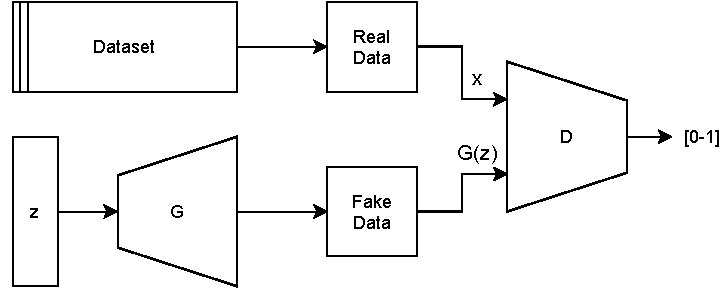
\includegraphics[width=0.8\textwidth]{chapters/GANs/figures/gan.pdf}
    \caption{Diagram of data use in training GANs}
    \label{fig:gan_diagram}
\end{figure}

To understand how these networks can learn, it is necessary to delve deeper into the theory and analyse how their loss function is defined. In the general sense, both the generator $G$ and discriminator $D$ are just functions of multiple variables. The generator is a map $G:\mathcal{Z} \to \mathcal{X}$, where $\mathcal{Z}$ is the latent space, defined by a probability distribution $p_{\bm{z}}$, and \gls{input_space} is the true data space, defined by a probability distribution $p_{data}$. The discriminator is a map $D:\mathcal{X} \to \mathbb{R}$ and $0 \leq D(\bm{x}) \leq 1$ (i.e. the probability of $\bm{x}$ belonging to the real data). In most practical cases $D$ and $G$ are implemented with neural networks, parameterized by $\bm{\theta}^{(D)}$ and $\bm{\theta}^{(G)}$ respectively.

The idea behind \acp{GAN} stems from Game Theory, where two agents compete against each other in a non-cooperative game \cite{improvedGANS2016}, the solution for this game is called the Nash equilibrium and in this situation both players have achieved their best expected value given the state of their adversary. Training a \gls{GAN} is a \textit{minimax} game that aims to reach the Nash equilibrium between the generator and the discriminator, the objective of these networks is given by \autoref{eq:gan_original_objective} \cite{gans2014}.
\begin{equation} \label{eq:gan_original_objective}
    \min_{G} \max_{D} V(D,G) =
    \mathbb{E}_{\bm{x}\sim p_{data}}\bigl\lbrack \log(D(\bm{x})) \bigr\rbrack + 
    \mathbb{E}_{\bm{z}\sim p_{z}}\bigl\lbrack \log(1 - D(G(\bm{z}))) \bigr\rbrack
\end{equation}

\autoref{eq:gan_original_objective} can be quite intimidating at first, but it is more easily understood by breaking it down into parts. First it is important to define what the symbol \gls{expected_value} means, this symbols represents the \textit{Expected value} of the operation between the square brackets. The expected value is a concept in statistics that means the average value that a variable will assume given some probability distribution, suppose for example rolling a 6-sided die, the expected value of the dice roll $n$ given the probability distribution $n\sim p_{dice}$ is given by \autoref{eq:expected_value_dice}.
\begin{equation} \label{eq:expected_value_dice}
    \mathbb{E}_{n\sim p_{dice}}(n) = \sum_{n=1}^{6}{n \cdot p_{dice}(n)} = 3.5
\end{equation}

More generally, the expected value $\mathbb{E}$ of a function $f(x)$, for all values $x$ following a probability distribution $p$, is represented as $\mathbb{E}_{x\sim p(x)}(f(x))$ (the use of square brackets in \autoref{eq:gan_original_objective} is not needed, it was only used to better separate the terms). This value is calculated as the sum of the values $f(x)$ multiplied by their respective probability given the distribution $p$. The general case for a finite probability distribution is represented in \autoref{eq:expected_value_discrete}.
\begin{equation} \label{eq:expected_value_discrete}
    \mathbb{E}_{x\sim p}\left( f(x) \right) = \sum_{i}{f(x_i) p(x_i)}
\end{equation}

When dealing with continuous probability distributions the summation in \autoref{eq:expected_value_discrete} is replaced by an integral, but in the context of machine learning most problems fall into the discrete category and the expected value is commonly approximated by calculating it from a mini-batch of data instead of the whole dataset.

With this understanding of expected value, it is possible to come back to the objective function in \autoref{eq:gan_original_objective}. Note that this is a minimax game, both the generator and discriminator are dependent on the same value $V(D,G)$, the discriminator tries to maximize the value, while the generator tries to minimize it. So the objective can be broken down into two loss functions $J^{(D)}$ and $J^{(G)}$, where each network is trying to minimize their own loss.

The objective of the discriminator is to maximize $V(D,G)$, this can be re-framed as a minimization problem over a loss function $J^{(D)} = -V(D,G)$ as mentioned by \textcite{nipsGAN2017}. So the loss for the discriminator is given by:
\begin{equation} \label{eq:discriminator_loss}
    J^{(D)}(\bm{\theta}^{(D)},\bm{\theta}^{(G)}) = 
    -\mathbb{E}_{\bm{x}\sim p_{data}}\left\lbrack \log(D(\bm{x})) \right\rbrack
    -\mathbb{E}_{\bm{z}\sim p_{z}}\left\lbrack \log(1 - D(G(\bm{z}))) \right\rbrack
\end{equation}

Observe what \autoref{eq:discriminator_loss} is saying, for the first term, $-\log(D(\bm{x}))$ will tend to infinity as $D(\bm{x}) \to 0$, the minimum value is $0$ for when $D(\bm{x})$ is exactly $1$; in other words, this term will be minimized when the discriminator correctly assigns the real data $\bm{x}$ as being $100\%$ real. The second term, $\log(1 - D(G(\bm{z})))$ will be minimized in the opposite way, when $D(G(\bm{z}))$ is equal to $0$; this means that this term encourages the discriminator to correctly assign the fake data as being fake.

The loss for the generator in the minimax game is simply the negative of the loss of the discriminator loss, $J^{(G)} = -J^{(D)} = V(D,G)$. One thing to note in the loss for the generator is that the first term of $V(D,G)$, as seen in \autoref{eq:gan_original_objective}, only depends on $D$, so it can be ignored since the generator can't affect the parameters $\bm{\theta}^{(D)}$. Then the loss for the generator can be written as the equivalent expression shown in \autoref{eq:generator_loss}.
\begin{equation} \label{eq:generator_loss}
    J^{(G)}(\bm{\theta}^{(D)},\bm{\theta}^{(G)}) = 
    \mathbb{E}_{\bm{z}\sim p_{z}}\bigl\lbrack \log(1 - D(G(\bm{z}))) \bigr\rbrack
\end{equation}

In this case, $\log(1 - D(G(\bm{z})))$ will be minimized when $D(G(\bm{z}))$ is equal to 1; in other words, the loss of the generator is minimized when the discriminator incorrectly classifies the fake data as being real, the generator is encouraged to reduce the discriminator accuracy.

One may wonder how can this game converge to producing a $p_{model}$ similar to $p_{data}$. To understand that, first it is necessary to understand how the difference between two probability distributions is measured. Much like distances between two points in space, that can be measured in different ways to produce different properties in that space (e.g. $\ell_2$ norm for the familiar Euclidean Space), there are multiple definitions of distance between probability distributions. Some definitions produce better properties that can be leveraged to solve particular problems, in the original \gls{GAN} proposal, \textcite{gans2014} proved that the objective given by \autoref{eq:gan_original_objective} is equivalent to reducing the distance called the Jensen-Shannon (JS) divergence.

The JS divergence is written in terms of another function, the Kullback-Leibler (KL) divergence. The use of the KL divergence can be found in many areas of machine learning, not just generative models, this is a very powerful metric that is closely tied to the concepts of information entropy and cross-entropy. The KL divergence between two probability distributions $p$ and $q$ is given by \autoref{eq:kl_divergence} \cite[p. 71-72]{deepLearningBook2016}.
\begin{equation} \label{eq:kl_divergence}
    D_{KL}(p \;\|\; q) =
    \mathbb{E}_{x\sim p}\left( \log\frac{P(x)}{Q(x)} \right) = 
    \sum_{x}{P(x)\left( \log\frac{P(x)}{Q(x)} \right)}
\end{equation}

One common characteristic between many metrics of distance for probability distributions is that they are not symmetric, that means that the distance between $p$ and $q$ is not the same as the distance between $q$ and $p$, this asymmetry is also present in the KL divergence as can be seen in \autoref{eq:kl_divergence} \textbf{--} it is for this reason that the name divergence is used instead of distance. Contrary to that, the JS divergence, although being called a divergence, is actually symmetric; it is defined in terms of the KL divergence as shown in \autoref{eq:js_divergence}.
\begin{equation} \label{eq:js_divergence}
    D_{JS}(p \;\|\; q) = \frac{1}{2}D_{KL}(p \;\|\; m) + \frac{1}{2}D_{KL}(q \;\|\; m) \qquad \text{where} \qquad
    m = \frac{p + q}{2}
\end{equation}

For both the KL and JS divergences, a value of 0 represents that the distributions $p$ and $q$ are the same, and minimizing these divergences brings the two distributions closer. As mentioned before, \textcite{gans2014} proved that the \gls{GAN} objective function given in \autoref{eq:gan_original_objective} minimizes the JS divergence and in turn should converge $p_{model}$ to $p_{data}$. The authors also proved that this convergence point equates to the optimal discriminator being unable to differentiate between real and fake data, having the same accuracy as a random guess ($50\%$).

The details of the proof are out of the scope of this document, the important information to take is how the networks reproduce the data distribution (by minimaxing the objective function) and why this works (equivalent to reducing the JS divergence). One important detail is that the proof relied on the fact that the updates to $G$ and $D$ were made directly in function space, the same argument does not apply to the situations seen in practice, where the updates to the functions are made on parameter space (i.e. $\bm{\theta^{(G)}}$, $\bm{\theta^{(D)}}$) \cite{nipsGAN2017}. This is not a problem in many situations, but there are multiple situations where this approach has been shown to diverge, or to cycle around the equilibrium without convergence; some examples of this are shown by \textcite{improvedGANS2016}, \textcite{wasserstein2017}, \textcite{wgan-gp2017} and \textcite{which_GAN_converge2018}.

One problem of minimizing the loss function of the generator $J^{(G)}$ as seen in \autoref{eq:generator_loss}, is that, in the start of training when the generator is still bad at producing results, the discriminator can become too good and will recognize the fake data with very high certainty; this confidence will saturate the discriminator output and give vanishing gradients for the generator updates, making training extremely slow. Given this problem, the original paper \cite{gans2014} proposed a change to the loss of the generator; instead of minimizing the probability of the discriminator being correct, the generator should maximize the probability of the discriminator making a mistake. This equates to minimizing the loss function shown in \autoref{eq:gan_logD_trick}.
\begin{equation} \label{eq:gan_logD_trick}
    J^{(G)} = -\mathbb{E}_{z\sim p_{z}}(\log D(G(\bm{z})))
\end{equation}

It is important to mention that this new loss function is an empirical recommendation, the theoretical arguments of convergence do not apply when training the generator with this function \cite{gans2014}. However, this does not seem to be a big problem in practical situations and is usually the preferred loss function between the two.

Another point worth mentioning is that for the theoretical argument of convergence, the generator updates would be made in relation with an optimal discriminator, this would mean that for each generator step, there should be multiple updates in the discriminator in order to have it be optimal for the current generator. At the beginning this was implemented as a new hyperparameter that would define how many updates to the discriminator would be made before updating the generator \cite{gans2014}, but later \textcite{principled_gan_methods2017} have shown that the optimal discriminator has gradient $0$ almost everywhere, making it impossible to train \acp{GAN} through gradient descent. This hyperparameter has since fallen out of fashion and usually \acp{GAN} are trained one step for each network, the original inventor of \acp{GAN} would also say: ``Many authors recommend running more steps of one player than the other, but as of late 2016, the author’s opinion is that the protocol that works the best in practice is simultaneous gradient descent, with one step for each player.'' \cite{nipsGAN2017}.

One may note how often the theory either fails to apply to practical cases or is replaced by empirical solutions that work better. This is very much the case not only for \acp{GAN}, but for many other areas of machine learning, ``[...] even though these [Artificial Neural Networks] are very useful tools based on well-known mathematical methods, we actually understand surprisingly little of why certain models work and others don’t'' \cite{visualizingFeatures2015}. In most \gls{GAN} methods introduced with a theoretical basis behind them, it is very common to see assumptions being made in order for the theorems proposed to apply \textbf{--} see for example the original \gls{GAN} paper \cite{gans2014}, or \cite{wasserstein2017} and \cite{TTUR_FID2017}.

\subsection{Mode Collapse}
One of the main problems faced when training \acp{GAN} is when the generator learns to map many, or all possible latent vectors in $\mathcal{Z}$ to the same point $\bm{x}$ in $\mathcal{X}$, this is called a mode collapse, also known as the ``Helvetica Scenario''. \textcite{nipsGAN2017} says that complete mode collapse is the most common form of harmful non-convergence in GANs and that, although complete collapse is rare, partial collapse is a frequent occurrence.

As an example of mode collapse, consider the case of training a \gls{GAN} to generate the handwritten digits of \gls{MNIST}, the generator collapsing could be that it only produces the number $6$ for all latent vectors, it may produce convincing results, but it can't represent the full distribution. This in theory could be useful, since new generators could be trained for each separate mode of the data (e.g. one generator for each digit). However this is usually not desirable, still considering the \gls{MNIST} example, after many iterations the discriminator would learn to be more suspicious of the number $6$ and the generator would then try to find a next mode to collapse (e.g. the number $8$); thus, both networks would be forever stuck changing modes and never reaching convergence \cite{improvedGANS2016}.
\begin{figure}[hbt]
    \centering
    \caption{Mode collapse on \gls{MNIST}}
    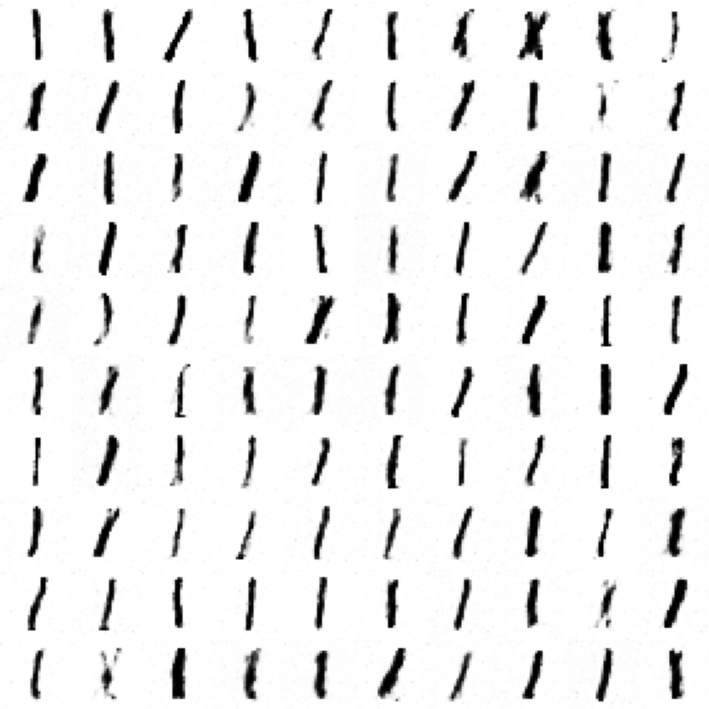
\includegraphics[width=0.5\textwidth]{chapters/GANs/figures/mode-collapse.png}
    \fonte{From the author (2021)}
    \label{fig:mode_collapse_mnist}
\end{figure}

\autoref{fig:mode_collapse_mnist} shows an example of extreme mode collapse that can happen when training \acp{GAN}, in this particular case the generator is a simple neural network of fully connected layers, having a single hidden layer, and being trained on the \gls{MNIST} dataset\footnote{
    When producing this image, the networks were trained four different times with different sets of hyperparameters, and in all cases the mode collapse happened on the number 1. This probably indicates that this is the easiest pattern for the generator to learn, but most importantly, it gives another counterargument on why it is usually not desirable to train several networks one for each mode, since it is difficult to produce the correct mode.
}.


\section{Proposed improvements}
Since their introduction in 2014, \acp{GAN} have become very popular for their capabilities but also for their difficult of being trained \cite{wgan-gp2017} and evaluated \cite{principled_gan_methods2017}. Many improvements have been proposed, of note between them are changes that aim to make training more stable and faster, reduce the effect of mode collapse, produce better results, scale the results to higher resolutions (in case of images), make the latent space have nicer properties, introduce new metrics of quality, and condition the generator on some know input in order to guide the generation process.

This section will explore some of the more popular methods, this is by no means an exhaustive list, the goal is only to introduce the techniques that were part of the empirical experiments in this document (see \autoref{cha:experiments}).

\subsection{DCGAN}
\glsreset{DCGAN}
The original \gls{GAN} suffered from training stability and difficulty of scaling to larger resolutions (in the case of images), \textcite{dcgan2015} were able to compile different popular techniques at the time to produce an architecture for the generator and discriminator that would produce better results and be more stable. They called this type of model a \gls{DCGAN} since they abandoned the use of fully connected and pooling layers in favor of using only convolutional and transposed convolutional layers.

Different from the other proposed improvements that will be mentioned later, the \gls{DCGAN} did not introduce any new way of training or using the data differently, it was simply a clever style of architecture that would produce better results. But the results were indeed very good, so much so that by 2016 most \gls{GAN} architectures were at least loosely based on the \gls{DCGAN} \cite{nipsGAN2017}.

The overall architecture can be summarized as follows \cite{dcgan2015}:
\begin{itemize}
    \item No fully connected hidden layers and no pooling layers overall, only uses convolution or transposed convolutions to change the dimensions of the input.
    \item Use of Batch Normalization in all layers of both networks, except the input layer of the discriminator and output layer of the generator.
    \item Use LeakyReLU for all layers of the discriminator and ReLU for all layers of the generator, use only \gls{tanh} in the last layer of the generator in order to produce the normalized images (i.e. interval $[-1, 1]$).
    \item Use of the Adam optimizer
\end{itemize}

\textcite{dcgan2015} were able to have stable training with the \gls{DCGAN} on a range of different datasets, the architecture was also robust enough to allow for building deeper models and generating higher resolutions. They also showed a surprising property by applying arithmetic on the latent space $\mathcal{Z}$, by taking some random latent vectors that would produce images of mans with glasses and averaging them, the result would be an average vector $\bm{z}(\text{``man with glasses''})$ that would represent this type of image; by also calculating $\bm{z}(\text{``man without glasses''})$ and $\bm{z}(\text{``woman without glasses''})$, and combining the vectors in the following way $\bm{z}(\text{``man with glasses''})$ - $\bm{z}(\text{``man without glasses''})$ + $\bm{z}(\text{``woman without glasses''})$, the result would be a latent vector that when fed to the generator would produce an image of a woman with glasses.

\subsection{Conditional GAN} \label{sub:cgan}
\glsreset{CGAN}
One of the main advantages of \acp{GAN} is that they can be trained with unlabeled data, this allows for learning with millions of real samples, such a volume of data is almost always very expensive and time consuming to have labelled. However, one of the earliest proposal for improvement was made by \textcite{conditionalGAN2014}, they argue about the benefits of leveraging the labels when training the \acp{GAN}.

This approach is conceptually very simple, when training the original \gls{GAN} the generator is fed some noise vector from $\mathcal{Z}$ and produces a fake sample $G(\bm{z})$, the discriminator then takes this and another real sample $\bm{x}$ to produce $D(G(\bm{z}))$ and $D(\bm{x})$. For a \gls{CGAN}, everything is the same except for the fact that both the generator and discriminator are also given a label $\bm{y}$ for the data generated; this means that the generator will produce $G(\bm{z} | \bm{y})$ and the output of the discriminator will be $D(G(\bm{z} | \bm{y}))$ and $D(\bm{x | \bm{y}})$.

The logic behind this approach is that it encourages the generator to learn how to distinguish the data as people do, \textcite{nipsGAN2017} comments that this may help the generator in optimizing the solution, but it also could be that the results produced are not necessarily closer to the real distribution, but instead that they favor characteristics that appeal to the human vision.

One advantage of this model is that it allows for more fine control over the result, in the unlabelled \gls{GAN} the results are random since they come from a sample of the latent space distribution; with \gls{CGAN} the label input can be used to set the class of the output, while the latent vector can be sampled multiple times to produce variation.

A question about the implementation of \acp{CGAN} is: how the label can be incorporated into the latent vector and the input image? In the original paper, \textcite{conditionalGAN2014} had the labels be represented as one-hot encoded vectors. For the generator the input $\bm{z}$ and the label vector $\bm{y}$ would be mapped into two layers of 200 and 1000 neurons respectively, these layers would then be combined into another layer that would have the label information imbued. A similar process would happen for the discriminator, it would map both the input and label into two one-dimensional layers and combine them into a new layer.

This way of combining the label with the data has mostly been replaced since then. A better way of doing that is to use embedding layers to represent the class label instead of one hot vectors, this layer should be mapped with a dense layer to a higher dimension and be reshaped into a channel of the input volume to the corresponding network (i.e. generator or discriminator). \autoref{fig:cgan} shows a diagram of how the label is incorporated into the channels using embedding layers. 
\begin{figure}
    \centering
    \caption{Generator and discriminator networks for \gls{CGAN}}
    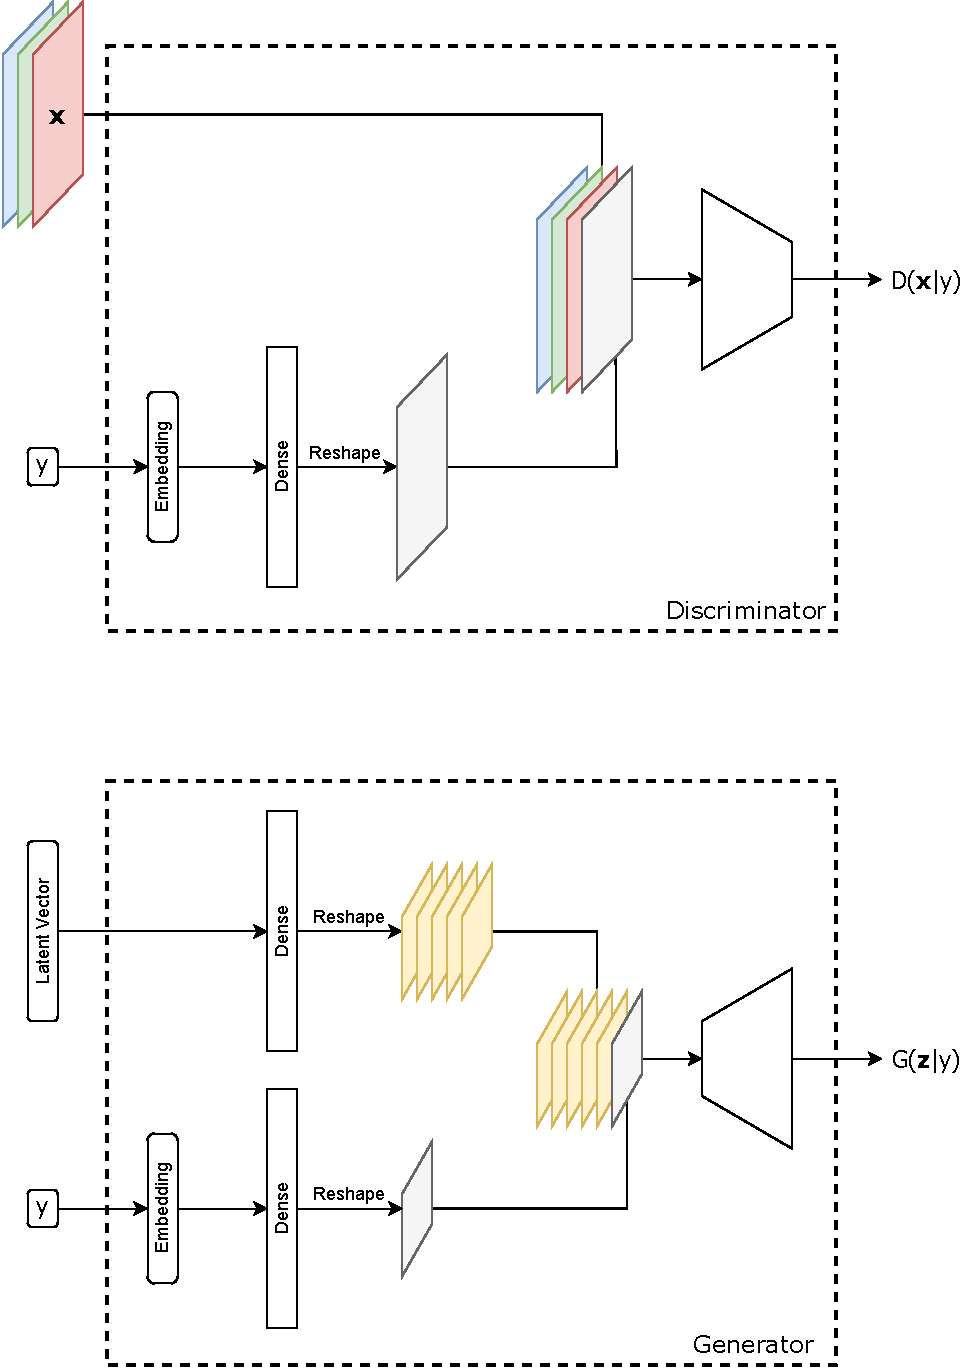
\includegraphics[width=0.8\textwidth]{chapters/GANs/figures/cgan.pdf}
    \fonte{From the author (2021)}
    \label{fig:cgan}
\end{figure}

\subsection{Wasserstein GAN} \label{sub:wgan}
One of the problems when training \acp{GAN} by trying to minimize the Jensen-Shannon divergence is that this metric does not produce the best gradients for the generator to learn, recall that \textcite{principled_gan_methods2017} have showed that for the optimal discriminator the gradient is equal to $0$ almost everywhere. The authors also explain that the Kullbak-Leibler divergence is also problematic since it can produce very high or very low values in different areas of the distributions, making training very difficult.

\textcite{wasserstein2017} introduce a simple example of a uniform probability for all points in the line segment $x=0$, $0 \leq y \leq 1$ on the $xy$ plane. They showed that any modeled distribution $x=\theta$ and $0 \leq y \leq 1$, that is parameterized by a single value $\theta$, will not converge when training with the JS, KL, and reverse KL divergences, or with the total variation distance\footnote{
    The details are out of the scope of this document, but the mathematical inclined reader is encouraged to check the original paper.
}. They propose the \gls{EM} or Wasserstein distance as an alternative to these other metrics and showed that in the proposed example, this distance produces a continuous value that provides usable gradients everywhere.

The motivation behind this choice of function is heavily inspired by theory. For this document most of the details will be omitted, and only the most relevant information will be quickly cited in order to reach the conclusions and information about the practical implementation. The \gls{EM} distance between two probability distributions $p$ and $q$ is defined by \autoref{eq:em_distance_scary}, ``where $\Sigma(p, q)$ denotes the set of all joint distributions $\gamma(x, y)$ whose marginals are respectively $p$ and $q$'' \cite{wasserstein2017}.
\begin{equation} \label{eq:em_distance_scary}
    W(p, q) = \inf_{\gamma \in \Sigma(p, q)} \mathbb{E}_{(x,y)\sim\gamma}\left\| x - y \right\|  
\end{equation}

In this equation the \textit{infimum} ($\inf$) can be interpreted as the greatest lower bound, so the \gls{EM} distance is given by the $\gamma$ distribution that satisfies the greatest lower bound condition for the corresponding expected value. There is an intuitive interpretation of this distance in terms of real world mechanics, consider that $p$ and $q$ describe two mass distributions with equal total mass, then the Wasserstein distance is equivalent to the minimum amount of energy necessary to move the masses around in order to transform the distribution $p$ into $q$, for this reason that it is also called the Earth Mover distance.

Calculating this distance in this form is extremely difficult, but by using the Kantorovich-Rubinstein duality the original authors rewrote the distance as shown in \autoref{eq:em_distance} \cite{wasserstein2017}.
\begin{equation} \label{eq:em_distance}
    W(p, q) = \sup_{\|f\|_{L} \: \leq \: 1}{
        \mathbb{E}_{x\sim p}f(x) - \mathbb{E}_{x\sim q}f(x)
    }
\end{equation}

The \textit{supremum} ($\sup$) in this equation is also interpreted as the least upper bound and the restriction $\|f\|_{L} \: \leq \: 1$ indicates that $f$ must be 1-Lipschitz continuous. A function $f$ is said to be K-Lipschitz continuous for a constant K when the following inequality holds \cite{lipschitz20XX}.
\begin{equation}
    | f(x) - f(y) | \leq K | x - y |  \qquad \forall x,y
\end{equation}

The inequality above can be interpreted as sliding a cone with inclination $K$ on every point of $f$ and if all the values of the function are outside the cone then the function is K-Lipschitz continuous.

\textcite{wasserstein2017} note that the 1-Lipschitz continuity can be replaced by a K-Lipschitz restriction while still maintaining the correct EM distance up to a multiplicative constant $K \cdot W(p,q)$. They also consider solving an easier problem by using a parameterized function $f_{\bm{\theta}}$, with $\bm{\theta}$ belonging to the parameter space $\Theta$, and replacing the $\sup$ with a $\max$. The simplified problem is given by \autoref{eq:em_distance_simpler}.
\begin{equation} \label{eq:em_distance_simpler}
    \max_{\bm{\theta} \in \Theta} {
        \mathbb{E}_{x\sim p}f_{\bm{\theta}}(x) - \mathbb{E}_{x\sim q}f_{\bm{\theta}}(x)
    }
\end{equation}

This simplified problem relies on the assumption that the supremum can be found for some set of parameters $\bm{\theta}$, but if this is true, then the \gls{EM} distance can be calculated (up to a multiplicative factor) by implementing $f$ as a neural network and using gradient ascent to maximize the value in \autoref{eq:em_distance_simpler} \cite{wasserstein2017}.

To better understand how this works, the problem in \autoref{eq:em_distance_simpler} can be written in terms of $p_{data}$, $p_{model}$ and a generator $G$ as shown in \autoref{eq:em_distance_critic}.
\begin{align} \label{eq:em_distance_critic}
    & \max_{\bm{\theta} \in \Theta} {
        \mathbb{E}_{\bm{x}\sim p_{data}}f_{\bm{\theta}}(\bm{x}) -
        \mathbb{E}_{\bm{x}\sim p_{model}}f_{\bm{\theta}}(\bm{x})
    } = \nonumber \\[10pt]
    & \max_{\bm{\theta} \in \Theta} {
        \mathbb{E}_{\bm{x}\sim p_{data}}f_{\bm{\theta}}(\bm{x}) -
        \mathbb{E}_{\bm{z}\sim p_{\bm{z}}}f_{\bm{\theta}}(G(\bm{z}))
    }
\end{align}

One may wonder where is the discriminator in all of this, the astute reader may have already realized that the discriminator is the function $f$. For the \gls{WGAN} however, the output of this function is not a probability but instead it can be any number; the interpretation is that the discriminator is scoring the data that it sees, so it is more commonly referred to as the \textit{critic}.

The goal of the critic is to approximate the \gls{EM} distance between the data and model distributions $W(p_{data}, p_{model})$, and it does that by maximizing the value in \autoref{eq:em_distance_critic}. How can the generator use this to learn a good probability distribution?

Since the goal of the generator is to minimize the distance between the real and modeled distributions, it's objective should be to minimize the value produced by the critic. \textcite{wasserstein2017} proved (theorem 3 of paper) that the gradient of the \gls{EM} distance for a generator parameterized by $\bm{\theta}$ is given by \autoref{eq:wgan_generator_grad}.
\begin{equation} \label{eq:wgan_generator_grad}
    \nabla_{\bm{\theta}} W(p_{data}, p_{model}) = -\mathbb{E}_{\bm{z}\sim p_{\bm{z}}}{
        \left\lbrack \nabla_{\bm{\theta}}f(G(\bm{z})) \right\rbrack
    }
\end{equation}

Although the theory is very heavy, the implementations changes are rather simple. The loss for the critic will be just the mean of the fake outputs $f(G(\bm{z}))$ minus the mean of the real outputs $f(\bm{x})$; in simpler terms, by minimizing this loss the critic is trying to give high scores for the real data and low scores for fake data. On the other hand, the loss for the generator is simply the negative mean of the fake outputs $f(G(\bm{z}))$, by minimizing this loss the generator is trying to maximize the score that the critic gives to the data that it produces.

One detail that was left to the side until now is the condition that the critic must be a K-Lipschitz continuous function, this is essential in order for the distance approximation to be valid and it is something that is not restricted by normal implementations of neural networks. The solution proposed by the authors was \textit{weight clipping}, that is, limiting the parameters of the critic to a interval $\left\lbrack-c, c\right\rbrack$ where $c$ is a constant hyperparameter. This is rather an unrefined solution, even the authors recognized that ``weight clipping is a clearly terrible way to enforce a Lipschitz constraint'' \cite{wasserstein2017}, but it was their best solution at the time and they encouraged further research to find a better way; and this improvement came in the form of a gradient penalty, in the next section this method will be explored further.

\subsection{WGAN with Gradient Penalty} \label{sub:wgan_gp}
One drawback about the \gls{WGAN} method is the hard restriction on the critic's parameters by way of weight clipping, this not only introduces a new hyperparameter $c$ that determines the clipping interval, but also leads to optimization difficulties as shown by \textcite{wgan-gp2017}; they demonstrated that when training, the gradients can either explode or vanish if $c$ was not carefully chosen, and that the critic is biased to much simpler functions.

\textcite{wgan-gp2017} proposed a new method to restrict the critic without needing to resort to hard clipping of the parameters. They base their technique by showing that the 1-Lipschitz function $f$ on \autoref{eq:em_distance} has a gradient of norm equal to $1$ almost everywhere under the distributions $p$ and $q$. Using this information, the loss function for the critic can be regularized to penalize for gradients that have norm far from $1$, thus the name \gls{WGAN-GP}. \autoref{eq:wgan_gp_loss} shows the regularized loss for the critic.
\begin{equation} \label{eq:wgan_gp_loss}
    J^{(C)} = \LaTeXunderbrace{\strut
        \mathbb{E}_{\bm{z}\sim p_{\bm{z}}} {\bigl\lbrack f(G(\bm{z})) \bigr\rbrack} - 
        \mathbb{E}_{\bm{x}\sim p_{\bm{data}}} {\bigl\lbrack f(\bm{x}) \bigr\rbrack}
    }_{\text{WGAN critic loss}} +
    \LaTeXunderbrace{
        \lambda\:\mathbb{E}_{\hat{\bm{x}}\sim p_{\bm{x}}} {
            \left\lbrack (\| \nabla_{\hat{\bm{x}}}f(\hat{\bm{x}})\|_{2} - 1)^{2} \right\rbrack
        }
    }_{\text{Gradient Penalty}}
\end{equation}

For this loss function, $\lambda$ is a new hyperparameter that defines the strength of the penalty (the original paper suggested that $\lambda = 10$ was a good value that applied to many situations), the probability distribution $p_{\bm{x}}$ is a uniform probability in the line between one real sample $\bm{x}$ and one fake sample $G(\bm{z})$, and $\hat{\bm{x}}$ is a sample from this distribution. What this means is that the gradient penalty is calculated by taking, for each pair of real and fake samples, a random point in the linear interpolation between them, and calculating the gradient of the critic with respect to this interpolation. Since the penalty is calculated per individual pairs, the critic should not use batch normalization since that would interfere with the penalty value, \textcite{wgan-gp2017} recommend using layer normalization as an alternative.


\subsection{Other techniques}
The experiments in this document also tried some other methods that will be described more briefly here.

\subsubsection{Style-based GAN}
This is the technique used in the StyleGan \cite{styleGAN2018} architecture, it proposes that the latent space $\mathcal{Z}$ be mapped to another space $\mathcal{W}$ using another neural network, and adding the mapped vector $w \in \mathcal{W}$ to the generator in a style-based fashion using only their mean and variances. This type of generator produced very high quality results in a variety of different datasets and the details of it's implementation are much more elaborate, but the simplified model built in the experiments was not fully explored and failed to produce good results; so for the sake of brevity, only this short explanation will be given.

\subsubsection{One Sided Label Smoothing}
Adding noise to labels is an old technique that has been proved useful in different areas of machine learning, in the context of \acp{GAN} it would change the objective of the discriminator from assigning the values $0$ for fake data and $1$ for real data, to a smoothed version like $0.1$ and $0.9$ for fake and real respectively.

However, \textcite{improvedGANS2016} have shown that smoothing the fake labels would cause problems for convergence in some areas of the probability distribution, so they recommending smoothing only the real label.

\subsubsection{Upsampling Methods}
The basic building block for upscaling the image in the generator for the \gls{DCGAN} is the transposed convolution layer, however, \textcite{deconvolutionArtifacts2016} have shown that this type of upsampling causes checkerboard artifacts in the images and recommend instead using a normal bilinear or nearest neighbour upsampling, followed by a normal convolutional layer. The experiments in this document tried comparing these three types of upsampling for different \acp{GAN} and datasets.


\section{Evaluating GANs} \label{sec:measure_gans}
\acp{GAN} are not only difficult to train, but also to evaluate. Consider for example two different \acp{GAN} that produce the handwritten digits of \gls{MNIST} and the desire is to compare them to see which one produces the more realistic or more varied results, how would one achieve such task?

Comparing two classifiers is relatively easy, the most natural way is just to observe their accuracy in the test dataset and see which one is higher. For \acp{GAN} on the other hand this is not so simple, remember that \textcite{gans2014} proved that the optimal discriminator would be unable to distinguish between real and fake data, and thus would have an accuracy of 50\%. But simply aiming for this value of accuracy would not work, since a discriminator that tosses a coin to decide would in fact produce the same value.

For many image generation applications, the most important aspect is to produce samples that are appealing to the human eye, so ultimately, a qualitative analysis made by people is very important. However, this is not a reliable measure of quality, \textcite{improvedGANS2016} have observed that workers on Amazon Mechanical Turk would produce varied results and the simple act of giving feedback would influence their accuracy; the authors also noted that they could easily distinguish real from the fake data produced by their models trained on the \gls{CIFAR}-10 dataset (over $95\%$ accuracy), while the workers would make mistakes much more frequently ($78.7\%$ accuracy).

Another problem of human evaluation is the fact that it is not so easy for a person to detect the variation of the model, the generator might produce very good samples while in a mode collapse state. The challenge is to evaluate not only the quality of individual samples, but also the variation over many samples. This is very challenging problem that still is not completely solved, being an active area of research, with new metrics still being proposed \textbf{--} see for example \cite{new_gan_metric_1} and \cite{new_gan_metric_2}. One yet unmentioned advantage of the \gls{WGAN} loss is that it can also be used to evaluate the models, the value of the \gls{EM} distance has been shown to correlate with the quality of the image generated \cite{wasserstein2017}.

Currently, two of the most popular metrics are the \gls{IS} and \gls{FID}, while the \gls{IS} has largely been replaced by \gls{FID}, both show good correlation with the image quality and also with image variety. For this document these were the two metrics used to evaluate the models in the experiments.

\subsection{Inception Score}
Just like a classifier can be used to predict the class of the test dataset, it can also be used to predict artificially generated images. If the classifier has a good accuracy, then it would make sense for it to be able to classify generated data with high confidence, given that this data is similar to the real data. This is the idea behind the \gls{IS}, bad samples would make a classifier be unsure of the right class, while good samples would produce very confident classifications.

In more defined terms, the value of how confident a classifier is that some input $\bm{x}$ belongs to a class $y$ is the conditional probability of $p(y | \bm{x})$, the idea is to calculate this over all labels $y$, and this value ideally should have a clear spike at some $y$, representing a high confidence classification\footnote{
    It's out of the scope of this document, but for those aware of the concept, the desired distribution should have low entropy
} \cite{improvedGANS2016}. By just measuring this value it would be possible to have an idea of the quality of the generated samples by the confidence of the classifier, but this alone would not be enough to detect the variety of the model, it is desired that the generator create samples in all classes, without giving preference to any particular label. This is equivalent of saying that $p(y)$ should be as uniform as possible\footnote{
    Equivalent to high entropy
} \cite{coursera_IS}.

By combining these two ideas, the \gls{IS} is calculated from the KL divergence between these two probability distributions as shown in \autoref{eq:inception_score}, note that the exponential operator is used only to make the numbers easier to interpret \cite{improvedGANS2016}.
\begin{equation} \label{eq:inception_score}
    \IncScore = \exp\bigl({\mathbb{E}_{\bm{x}\sim p_{model}}{
        \bigl\lbrack D_{KL}(p(y | \bm{x}) \;\|\; p(y)) \bigr\rbrack
    }}\bigr)
\end{equation}

Since the desired behaviour is for $p(y | \bm{x})$ to be very well defined at a single point while $p(y)$ should be completely uniform, then the KL divergence between those two should be as high as possible, this means that for the \gls{IS}, higher values means better results. To calculate the expected value expected value it is necessary to average the results over many generated samples in order to have a close approximation of the true value, the original authors used $50,000$ in their experiments \cite{improvedGANS2016}.

The remaining detail is what classifier to use when calculating the \gls{IS}, this metric uses the Inception v3 model \cite{inceptionV3_2015}, hence the name Inception Score. The Inception model is a very powerful model trained on 1000 classes of the ImageNet dataset of natural images, so it is very sensible as the classifier of choice. There are however some limitations, since the model was trained on ImageNet it may not offer good classification for datasets that are too different from natural images (like \gls{MNIST}) or from the 1000 classes learned.

Other shortcomings of the \gls{IS} are that it could give very high scores for models that generate only a single good image for each category (a form of mode collapse) and that it also completely ignores the training dataset (the very thing that the generator is trying to model) \cite{coursera_IS}.


\subsection{Fréchet Inception Distance}
The \gls{FID} metric was introduce as an improvement over the previous \gls{IS}, it was shown to correlate well with human perception and be more consistent than the \gls{IS} for different types of disturbances to the images (i.e. the \gls{FID} consistently gets worse as images get more disturbed, while the \gls{IS} fluctuates) \cite{TTUR_FID2017}.

The Inception v3 model is also used to calculate this metric, but instead of using the class predictions from the output layer like the \gls{IS}, the \gls{FID} uses features from the last global pooling layer. To understand why this is a useful choice it is important to know how computer vision models see the data. The idea behind deep learning models is that each layer of the network can capture a different level of abstraction in the data, for example, the layers start detecting edges, followed then by shapes, textures, and finally high level patterns. The Inception v3 model takes as input $299\times299\times3$ images and reduces them to a $1024$ dimensional vector of features, this is a compression of about $262$ times the original size; with such aggressive reduction it is imperative for the model to learn only the most relevant features, these are able to describe the data in a much more abstract level without being affected by unimportant things like small random noise.

For a well behaved model like Inception v3, if two images share similar feature vectors, they are probably very similar in an abstract sense as well. Two images of cats will have similar features, even more so if the cats have similar colors, pose or fur. By using the feature layer to measure the \gls{FID} it is possible to evaluate how well the model represents the structure of the data, and not punish it if it cannot reproduce the exact images of the training set.

The \gls{FID} uses another metric for the difference between probability distributions called the Fréchet Distance, the difference is calculated between the distributions of the feature vectors for the real and fake images. For practical purposes only the mean and covariance are considered, so it is assumed that the distributions follow a multidimensional Gaussian, making the \gls{FID} metric be calculated as shown in \autoref{eq:fid} \cite{TTUR_FID2017}.
\begin{equation} \label{eq:fid}
    \FID = \|\bm{\mu}_{data} - \bm{\mu}_{model}\|_{2}^{2} + 
    \Tr\bigl(\bm{V}_{data} + \bm{V}_{model} - 2(\bm{V}_{data} \cdot \bm{V}_{model})^{\frac{1}{2}}\bigr)
\end{equation}

In this equation $\bm{\mu}$ and $\bm{V}$ represent the mean vector and the covariance matrix for the feature vectors, calculated for a big enough sample of the real and fake data (i.e. $50,000$). The $\Tr$ operator calculates the trace of the matrix (i.e. the sum of all the elements of the main diagonal), and the matrix square root inside the trace is not calculated element-wise, it is instead the actual square root of the entire matrix. Since this metric is a distance between real and fake data and it is desirable for this distance to be small, then for the \gls{FID}, lower values means better results.

One of the main advantages of the \gls{FID} is that it considers the training dataset in the evaluation, so a better model would be the one who can better replicate the structure of the data used to learn. This metric is considered better than the \gls{IS} and has generally replaced it \cite{coursera_IS}, however it still suffer from some of the same shortcomings, notably the fact that it only works for evaluating \acp{GAN} in the image domain and that it still relies on the specifics of the Inception v3 model.

\subsection{Using other classifiers}
Although the original \gls{IS} and \gls{FID} rely on the Inception v3 model, the same metrics could be calculated using another classifier trained specifically for the data used in training the \gls{GAN} model \textbf{--} for this document this will be called the \gls{CS} and \gls{FCD} respectively \textbf{--} this can produce more accurate results for datasets like \gls{MNIST} that contain very different images from the ones in ImageNet used to train Inception v3.

One disadvantage of this approach is that it is not useful when comparing models evaluated with different classifiers, however it is always possible to fall back to the original \gls{IS} and \gls{FID} as a common ground for comparison, keeping in mind that these metrics may not be very accurate anyway depending on the dataset.

For the experiments in this document it was decided to train individual classifiers for each dataset in order to produce more accurate metrics, the comparisons with other published models was judged less relevant since the idea is to compare all the techniques experimented on, it falls off the main scope of this document to directly compare the results of other works. Also because for some of the older methods, the \gls{IS} and \gls{FID} metrics were not even introduced at the time.
